\documentclass[letterpaper]{article}
\usepackage[spanish,es-tabla]{babel}
\usepackage{indentfirst}
\usepackage[utf8]{inputenc}
\usepackage{graphicx}
\usepackage{amsmath}
\usepackage{amsfonts}

\usepackage[usenames,dvipsnames,svgnames,table]{xcolor} 

\title{ Trabajo Practico N$^\circ$2 \\ Economía }
\author{ Gatica, Isaias \\ Piñel, Julian \\ Saez, Lautaro Andres \\ Vidman, Xavier  }
\date{}

\begin{document}

\maketitle

\section{Ejercicio 4}

\subsection*{b}

Debemos demostrar que el cual la combinación de puntos que le otorga la máxima satisfacción dependiendo del presupuesto
tengo que el máximo va a ser el punto en el cual la curva de indiferencia dada tiene como tangente 
a la ecuación de la recta presupuestaria, para ello se aplicaran los multiplicadores de Lagrange.

\begin{equation}
\label{eq.U}
U(X,Y)=X^aY^b 
\end{equation}

La  de eq.\ref{eq.U} esta restringida a 

\begin{equation}
\label{eq.restriccion}
M = P_xX+P_yY
\end{equation}

Calculando la derivada de $U$ por regla de la cadena obtenemos

\begin{equation}
\label{eq.dU}
dU= \frac{\partial U}{\partial X}dx + \frac{\partial U}{\partial Y}dy
\end{equation}

Como se debe hallar los puntos críticos igualamos a 0, dando 
como resultado 

\begin{equation}
\frac{\partial U}{\partial X}dx = -\frac{\partial U}{\partial Y}dy
\end{equation}
    
Sabiendo que $\partial U/\partial X=UM_x$ y $\partial U/\partial Y=UM_y$ entonces

\begin{equation}
UM_xdx = -UM_ydy
\end{equation}

Despejando obtenemos 

\begin{equation}
\label{eq.dy1}
\frac{dx}{dy}=-\frac{UM_x}{UM_y}
\end{equation}

Por otro lado de la eq.\ref{eq.restriccion} se puede obtener 

\begin{equation}
y = \frac{M}{P_y} - \frac{P_x}{P_y}x
\end{equation}

Derivando 

\begin{equation}
\label{eq.dy2}
\frac{dy}{dx}=-\frac{P_x}{P_y}
\end{equation}

Por transitividad eq.\ref{eq.dy1}, eq.\ref{eq.dy2}

\begin{equation}
\frac{UM_x}{P_x}=\frac{UM_y}{P  _y}
\end{equation}

Es posible observas que las cantidades optimas para cada bien son
inversamente proporcionales a sus precios.

\section{Ejercicio 5}

Sabemos que la tasa de sustitución marginal (\textbf{TSM}) se puede calcular
como:

\begin{equation}
\label{eq.tmst}
TMS_{xy}=\frac{UM_x}{UM_y}
\end{equation}

donde $UM_j=\frac{dU}{dj}$

Entonces para la función 

\begin{equation}
U(X,Y)=Y + aX
\end{equation}

Se obtiene:

\begin{equation}
UM_x = a , UM_y = 1
\end{equation}

Por lo cual aplicando la eq.\ref{eq.tmst} se obtiene 

\begin{equation}
TMS_{xy}=a
\end{equation}

Como $\textbf{TMS}$ es constante, dado que $a>0$ cualquier aumento de la cantidad del bien $x$, producirá 
un aumento del bien $y$, lo cual nos indica que el bien $x$ y el bien $y$ son complementarios. 

\section{Ejercicio 6}

La función de utilidad es $U(x,y)=\frac{1}{2}xy$.

Sabemos que el punto de equilibrio del consumidor es cuando el intercambio de
bienes sea optimo según el presupuesto disponible y sus gustos, preferencias
se da gráficamente cuando la recta presupuestaria corta a la curva de indiferencia.

Analíticamente $M=P_xx+P_yy$, se sabe que el intercambio de bienes óptimos
se da cuando

\begin{equation}
TMS = \frac{P_x}{P_y} \lor \frac{U_x(x,y)}{U_y(x,y)}=\frac{P_x}{P_y} 
\end{equation}

entonces podemos obtener 

\begin{equation}
\frac{y}{x}=\frac{P_x}{P_y} \Rightarrow y=\frac{P_x}{P_y}x
\end{equation}

Reemplazando la ecuación anterior en $M=P_xx+P_yy$ obtenemos 

\begin{equation}
M=P_xx+\frac{P_yP_x}{P_y}x \Rightarrow M=2P_xx
\end{equation}

Finalmente obtenemos que la demanda de x

\begin{equation}
x=\frac{M}{2P_x}
\end{equation}

Por otro lado la demanda de y se puede expresar como 

\begin{equation}
y=\frac{M}{2P_y}
\end{equation}

Por lo tanto las coordenadas de punto de equilibrio son

\begin{equation}
(x;y)=\left( \frac{M}{2P_x} ; \frac{M}{2P_y} \right)
\end{equation}

\begin{figure}[h]
\centering
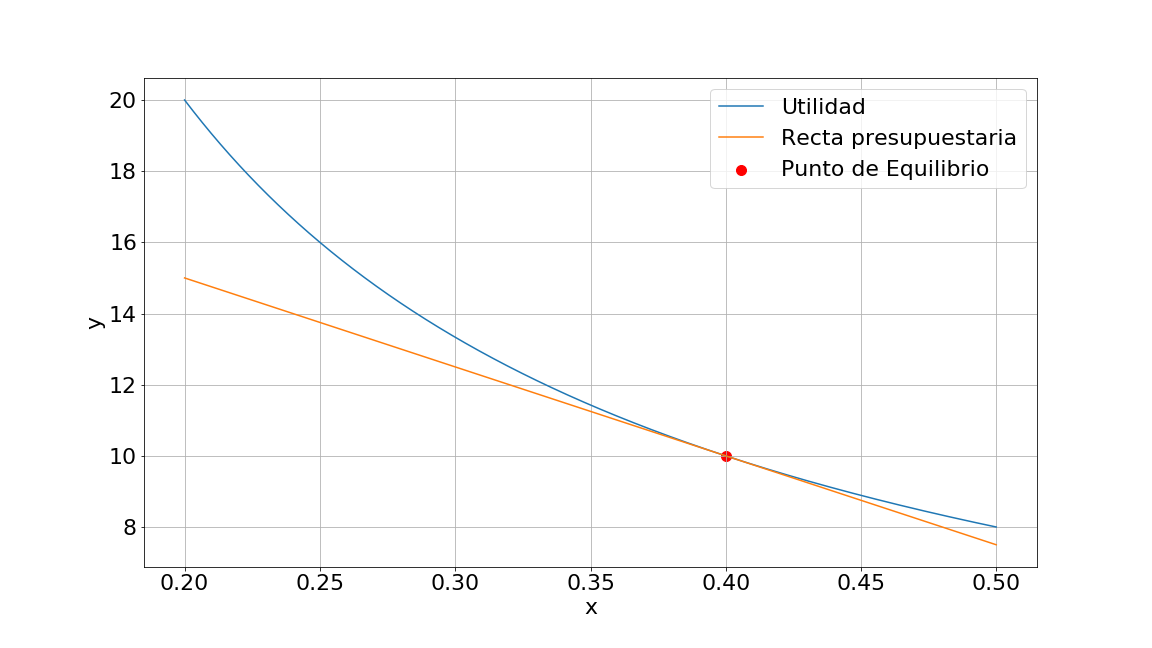
\includegraphics[width=\textwidth]{./Images/punto_6.png}
\caption{Representación gráfica del punto de equilibrio.}
\end{figure}

\section{Ejercicio 7}

\begin{equation}
U(x,y)=(xy)^{1/2} \land P_x=3 \land P_y=4
\end{equation}

Sabiendo que $M=90$ y luego $M=180$ obtenemos que 

\begin{equation}
M=P_xx+P_yy
\end{equation}

reemplazando por lo valores de $M$ obtenemos 

\begin{equation}
\label{eq.90}
y = \frac{90-3x}{4}
\end{equation}

\begin{equation}
\label{eq.180}
y = \frac{180-3x}{4}
\end{equation}

Buscamos el punto de equilibrio para los dos casos

\begin{equation}
\frac{U_x}{U_y}= \frac{P_x}{P_y}
\end{equation}

Obtenemos 

\begin{equation}
y= \frac{3}{4}x
\end{equation}

Para $M=90$

\begin{equation}
90=3x+4\frac{3}{4}x \Rightarrow 90=6x \Rightarrow x=15
\end{equation}

Reemplazando en eq.\ref{eq.90} se obtiene que $y=11.25$.

Por otro lado para $M=180$

\begin{equation}
180=3x+4\frac{3}{4}x \Rightarrow 180=6x \Rightarrow x=30
\end{equation}

Con la eq.\ref{eq.180} obtenemos $y=22.5$.

\newpage

\begin{figure}[h]
\centering
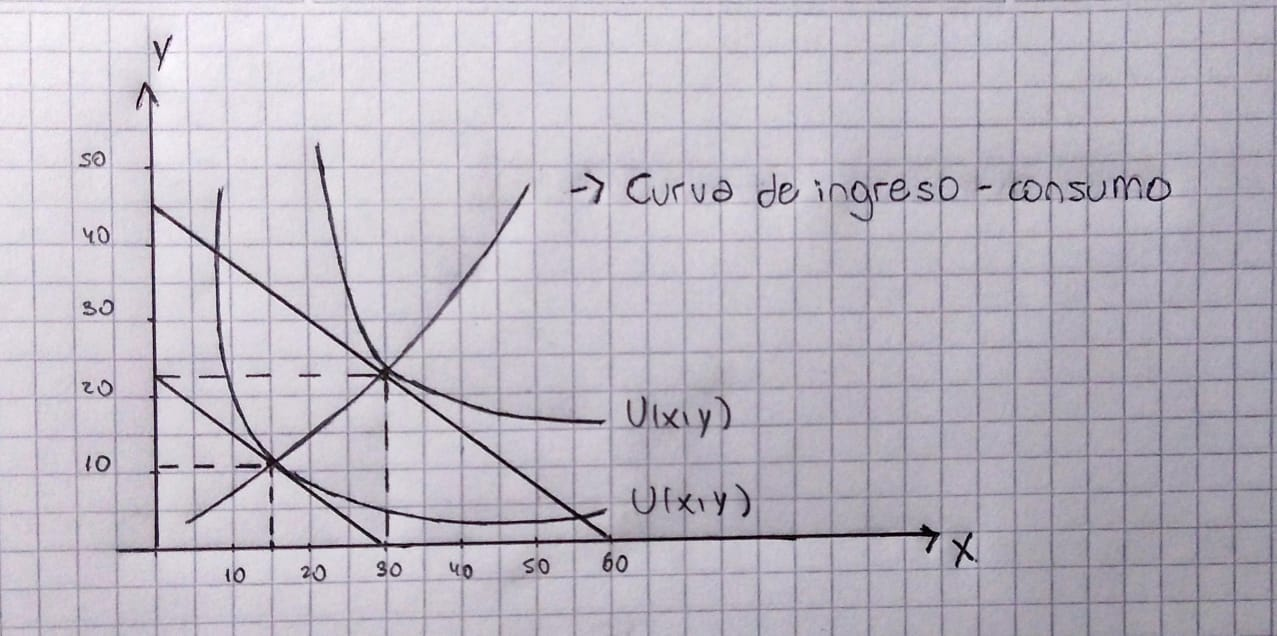
\includegraphics[width=\textwidth]{./Images/punto7.jpeg}
\caption{Método geométrico del obtención de punto de equilibrio.}
\end{figure}

\section{Ejercicio 8}

\subsection*{i}

Utilizando la eq.\ref{eq.tmst} se pudo completar la siguiente tabla.

\begin{table}[htbp]
\centering
\begin{tabular}{|c|c|c||c|c|c|}
\hline $Q_x$ & $Q_y$ & $TMS_{xy}$ & $Q_x$ & $Q_y$ & $TMS_{xy}$ \\ 
\hline 1     & 10    & ...     & 3     & 10    & ...     \\
\hline 2     & 5     & -5      & 4     & 7     & -3      \\ 
\hline 3     & 3     & -2      & 5     & 5     & -2      \\ 
\hline 4     & 2.3   & -0.7    & 6     & 4.2   & -0.8    \\ 
\hline 5     & 1.7   & -0.6    & 7     & 3.5   & -0.7    \\ 
\hline 6     & 1.2   & -0.5    & 8     & 3.2   & -0.3    \\ 
\hline 7     & 0.8   & -0.4    & 9     & 3     & -0.2    \\ 
\hline 8     & 0.5   & -0.3    & 10    & 2.9   & -0.1    \\ 
\hline 9     & 0.3   & -0.2    &       &       &         \\ 
\hline 10    & 0.2   & -0.1    &       &       &         \\ 
\hline
\end{tabular}    
\caption{Valores de $TMS_{xy}$ obtenidos.}
\end{table}

\section*{ii}

Sabemos que la recta presupuestaria es de la forma

\begin{equation}
M = P_xx+P_yy
\end{equation}

Sabemos que $M=10$, $P_x=P_y=1$ entonces

\begin{equation}
y=10-x
\end{equation}

Gráficamente la recta presupuestaria interfecta a la curva de indiferencia en $P=(5;5)$

\begin{figure}[htbp]
\centering
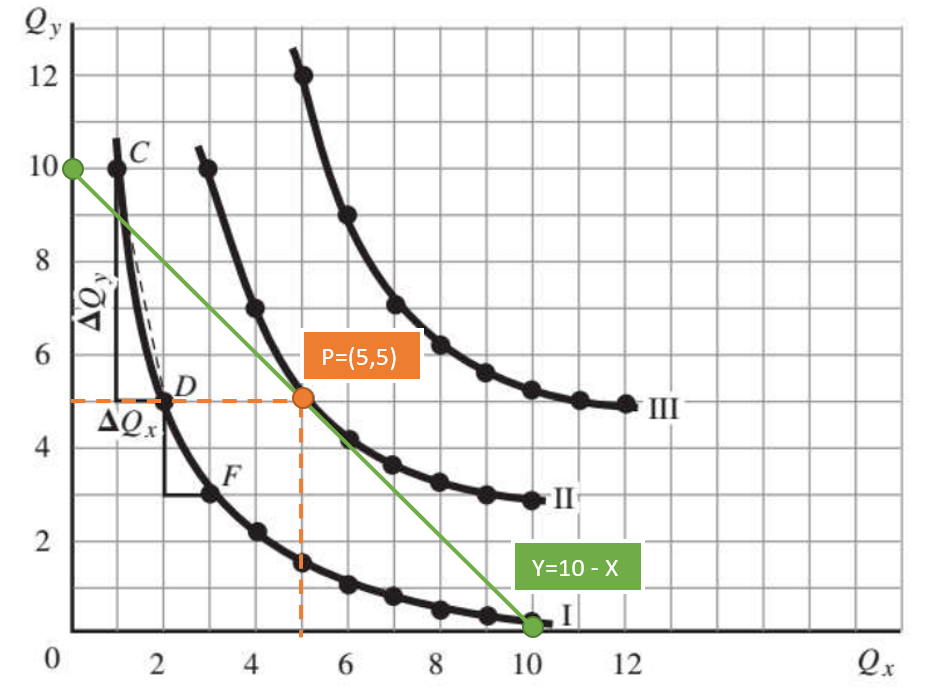
\includegraphics[width=\textwidth]{Images/punto_8.png}
\end{figure}

\end{document}